\chapter{Обзор литературы} \label{ch2}

Ввиду постановки задачи, текущая глава посвящена обзору существующих решений 
сразу двух направлений:
\begin{itemize}
    \item инструментов в LLM-агентах;
    \item автоматизации решении задач.
\end{itemize}

Начнем главу с первого направления.

\section{Обзор существующих реализаций инструментов} \label{ch2:sec1}

Прежде чем говорить о действиях, которые могут совершать LLM-агенты и MAS, нужно обозначить
то, как выглядят эти действия. Стоит понимать, что все действия - это вызов 
некоторой функции. Но вот то, как именно происходят вызовы - будет далее изложенно 
в этой секции.

\subsection{Определение классических вызовов инструментов} \label{ch2:sec1:subsec1}

Вызов инструментов, ровно как и работа LLM в формате чат-модели - свойство, достигаемое
обучению моделей на синтетических данных, которые внешне сильно отличаются от тех,
которые можно встретить как в интернете, так и в различных специфических источниках 
(например, разметках веб-страниц): примером такой разметки служит ChatML \cite{chatml}. В действительности, свойство модели 
``поддерживать'' разговор в формате диалога, ``вызывать'' инструмент - некоторого рода 
договорённость, по которой и модель понимает, как ей генерировать более точно ответ,
так и разработчики понимают, как обрабатывать результат. Именно эта договоренность
позволяет использовать LLM в качестве чат-бота или агента.

Стоит отметить, что вид разметки вызова инструмента можно 
формировать при помощи дополнительного описания в контексте, однако одним из часто испльзуемых
форматов все же остается JSON схема. Примером этого служит изображение \firef{fig:ch2:tool_invoke}. 
Это пример вызова инструмента и передаваемых параметров в специальной JSON разметке.

\begin{figure}
    \center
	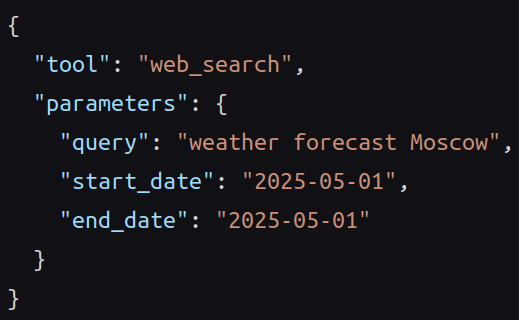
\includegraphics[scale=0.36]{sources/json_tool_invoke.png}
	\caption{Пример вызова LLM при запросе узнать погоду в Москве: 'tool' - название 
инструмента, 'parameters' - аргументы инструмента.} 
	\label{fig:ch2:tool_invoke}  
\end{figure}

Такие модели, в отличие от обычных моделей, которые лучше понимают, как вызывать 
инструменты, как обрабатывать некоторого рода запросы, носят специальные названия:
например, суффикс '-instruct'. Это важно отметить ввиду того, что от выбора модели 
зависит качество работы всей мультиагентной сети в целом. 

Как понятно из примера и теории выше, все аргументы и возвращаемые типы при
таких вызовах функций - данные текстовопредставимые: строки и числа. Это накладывает
ряд ограничений на инструменты: в такие функции нельзя передавать в явном виде типы,
которые в явном виде не представимы в виде строк (например, изображения, видео), 
ровно как и функции - должны возвращать строки. Но можно передавать их неявно: например,
через пути к файлам - в некоторых сценариях это допустимо.

Стоит отметить, что попытки передать изображения и видео в явном виде функциям при помощи 
LLM (например, в формате строки байт-кода) провальна: как минимум из-за того, что символы,
входящие в байт-код, могут не поддерживаться LLM. Максимально приближенным способом работы
с данными в условиях, когда они не могут быть предствлены в виде текста, можно использовать
различные большие фундаментальные модели, работающие с данными модальностями: например, 
VLM для работы с изображениями \cite{pixtral}. Такие модели, не смотря на некоторые
неточности, успешно проявляют себя в решении ряда задач \cite{vlm_in_charts}.

Последним, хоть и незначительным, но недостатком, является практическая особенность 
реализаций таких инструментов: хоть концептуально, вызовом действия может допускаться
вызов любой функции, в большинстве случаев многие полезные функции, которые были бы 
актуальны для агента, невозможно вызвать напрямую ввиду разногласий в реализациях 
интерфейсов. В таких случаях можно воспользоваться одним из двух вариантов:
\begin{itemize}
    \item реализовать адаптер для вызова метода с несовместимым для LLM интерфейсом;
    \item использовать готовый интерфейс коммуникации, например: MCP. 
\end{itemize}
О последнем далее и пойдет речь.

\subsection{Определение MCP-инструментов} \label{ch2:sec1:subsec2}

Не смотря на недостатки классических LLM-инструментов, их свойств достаточно для их
применения в широком круге задач. Этому соответствуют множество косвенных факторов, но
одним из них является выпущенная Anthropic унифицированный протокол взаимодействия с 
инструментами ModelContextProtocol (или MCP) \cite{mcp-docs}.

Вкратце, данный протокол позволяет модели обращаться и работать не только с внешними 
инструментами, но и с различными абстракциями в целом: это могут быть другие агенты и 
мультиагентные системы, источники знаний для генераций LLM-ответов с привлечением внешних 
источников (Retrieval Augmented Generation или RAG) и многое другое. Нам же это интересно
в первую очередь интерфейс из-за его возможности работать с инструментами.

На \firef{fig:ch2:mcp_survey} из \cite{mcp_survey}
представлен общий план агентной системы, работающей с инструментами MCP. Как видно из 
рисунка, для реализации подключения LLM-агента к некоторому инструментарию или
окружению через интерфейсы MCP необходимо реализовать MCP-клиент и MCP-сервер. 

\begin{figure}
    \center
	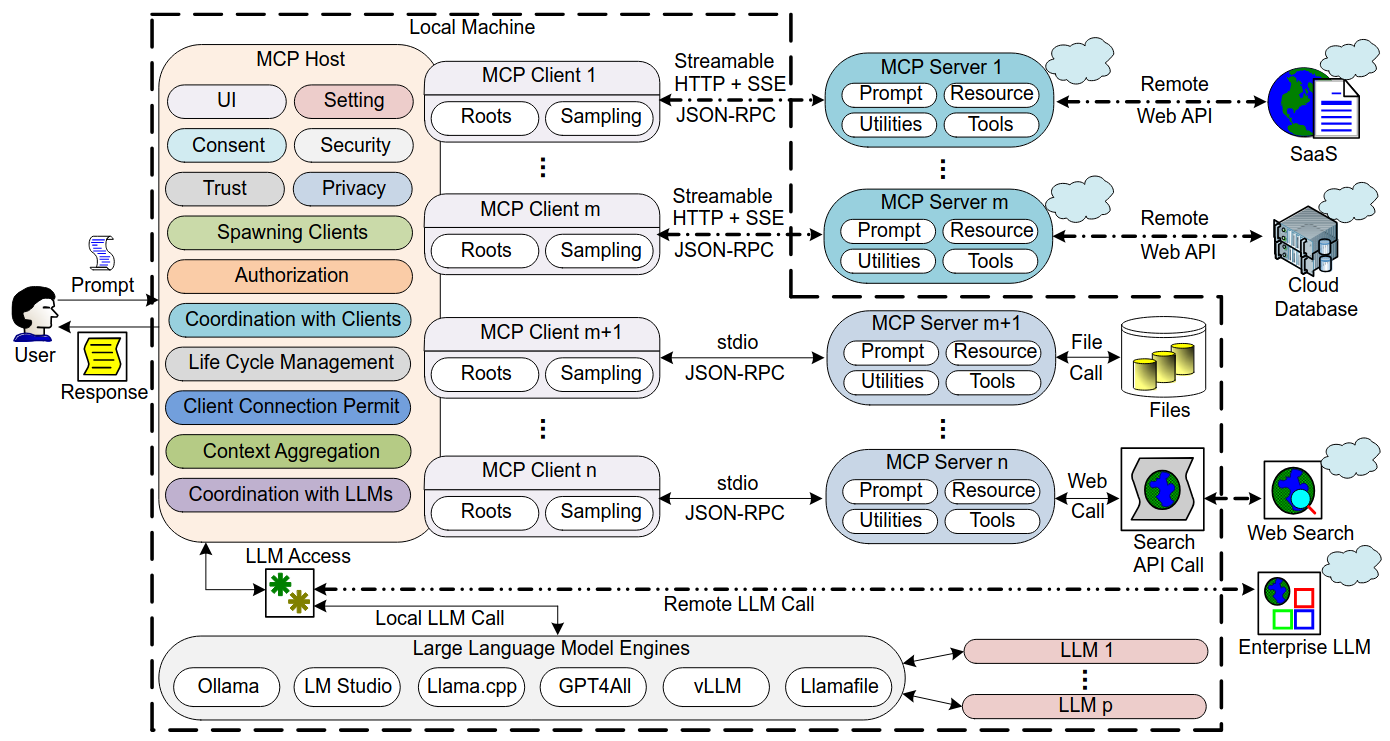
\includegraphics[scale=0.32]{sources/mcp_workflow.png}
	\caption{Полный цикл работы MCP протокола с LLM.} 
	\label{fig:ch2:mcp_survey}  
\end{figure}

Такая пара для каждого инструментария своя: она обеспечивает взаимодействие между 
LLM-агентом и инструментами. Все MCP-клиенты размещается на том же устройстве, 
на котором работает LLM-агент. MCP-сервера, напротив, не обязаны размещаться на том же 
устройстве, что и клиент: они могут быть как на локальном вычислительном устройстве и 
работать через stdio, так и удаленнымы, и работать через HTTP запросы. 
Это деталь важна для нас не с технической точки зрения, а с практической: MCP интерфейсы 
предлагают \textit{простое и гибкое} взаимодействие с окружениями разного уровня доступности: с локальными и 
удаленными.

Список открытых инструментов постоянно пополняется и его можно наблюдать в открытых
источниках: например, в официальном GitHub репозитории MCP \cite{mcp-servers}. 

Не взирая на все удобства MCP, данный интерфейс не устраняет недостатков для работы с 
данными других типов. Именно потому стоит рассмотреть другой вариант работы 
с инструментами.

\subsection{Определение кодовых инструментов} \label{ch2:sec1:subsec3}

Для работы с инструментами, требующие в явном виде данные отличных от текста модальностей,
можно воспользоваться свойством LLM-агентов генерировать код и пытаться исполнять его:
такое решение предложено авторами в статье CodeAct \cite{codeact}, к которому еще вернемся.
В данной работе предлагается генерировать вместо специфичного текста-разметки для выбора 
некоторого действия (или набора действий) сразу код, в котором могут присутствовать 
те же вызовы инструментов, но уже имеющие синтакс языка генераций. Процесс работы агента
с кодогенерацией и инструментами представлен на рис \firef{fig:ch2:codetools}.

\begin{figure}
    \center
	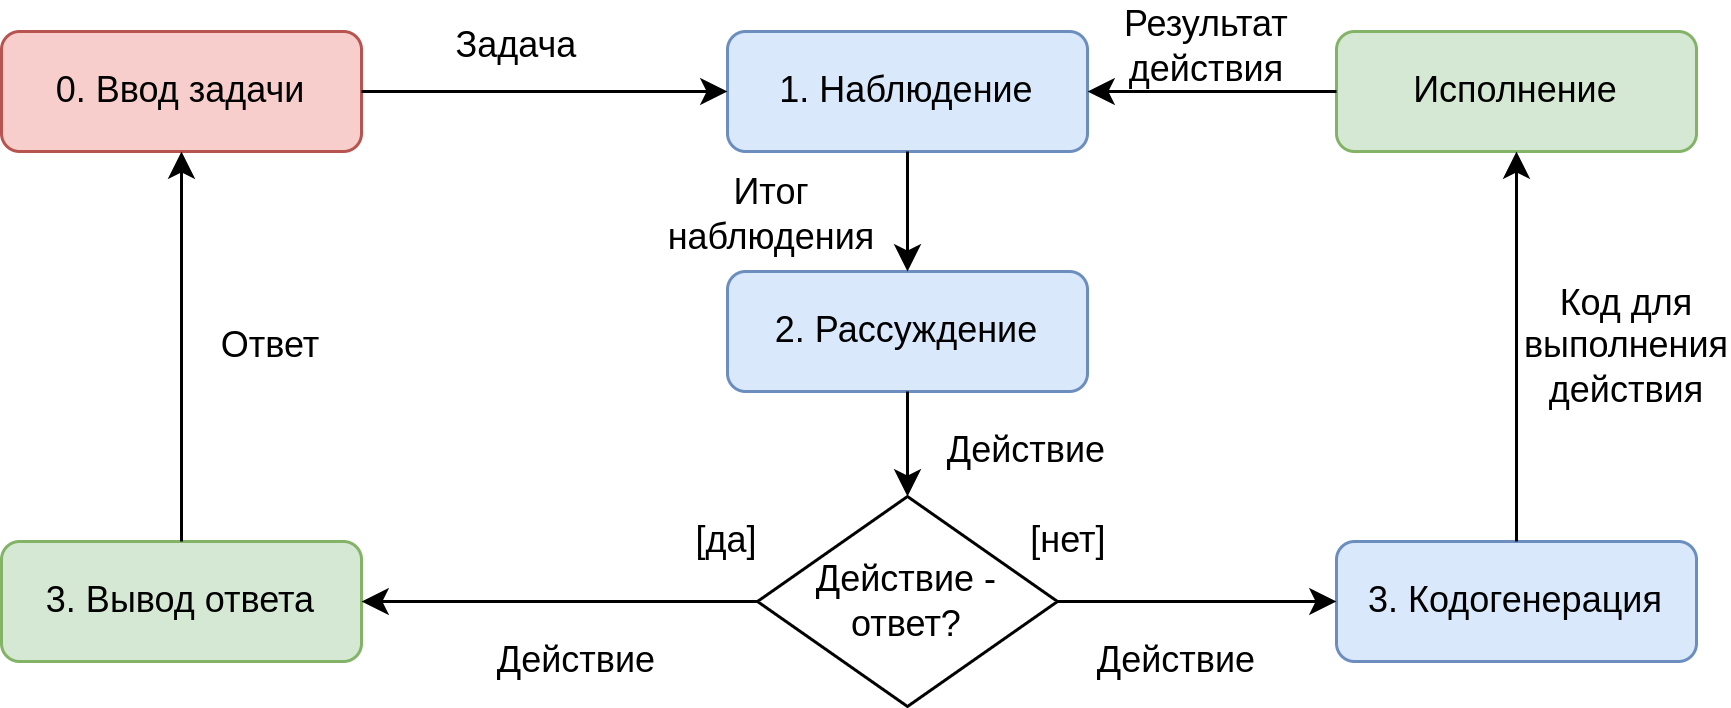
\includegraphics[scale=0.24]{sources/codeact_schema.drawio.png}
	\caption{Принцип работы CodeAct: вызов инструмента (действия) происходит в формате
кодогенерации на определенном языке программирования. Красные блоки - действия, 
выполняемые пользователем; синие - LLM; зеленые - кодом программы.} 
	\label{fig:ch2:codetools}  
\end{figure}

Такой подход предоставляет сразу несколько плюсов:
\begin{itemize}
    \item работа с различными типами данных: теперь диапазон допустимых инструментов
не ограничивается модальностями аргуемнтов и возвращаемого значения; 
    \item наличие логики в вызове инструментов: генерируемый код может иметь условные 
операторы, циклы, а также обрабатывать исключения - при условии если это все поддерживает
язык генерации кода.
\end{itemize}

У такого метода есть два недостатка:
\begin{itemize}
    \item \textit{безопасность}: хоть и существуют исследования касательно того, 
как делать генерацию и исполнения кода более безопасной, нет гарантий, что 
код не окажется вредоносным;
    \item \textit{мультимодальность}: такой подход позволяет вызывать инструменты, 
работающий с отличным от текстом типами данных, но в предлагаемом решении кодогенерация 
всё еще обязана генерировать только текст в качестве результата работы кода 
(например: вывод в терминал).
\end{itemize}

\subsection{Проблема большого количества инструментов} \label{ch2:sec1:subsec4}

Одна из проблем, с которой можно столкнуться в процессе разработки агентов - большое
количество инструментов. Эта проблема возникает из-за того, что всю подробную информацию
о названиях, свойствах и решаемых задачах инструментов необходимо указывать при запросах 
каждом запросе больших языковых моделей. Это вызывает сразу две проблемы:
\begin{itemize}
    \item увеличенный расход вычислительных мощностей: современные LLM 
основаны на базе архитектуры ``трансформеров'', которые производят матричные перемножения,
одна из размерностей которых фиксирована, а другая - имеет длину входного текста.
Потому эти модели имеют квадратичную сложность $O(N^2)$ от длины входного запроса (эта
сложность или временная \cite{attn_need}, или по памяти за счет кэширования и 
оптимизаций\cite{cached_kv} - зависит от реализации).
    \item ухудшение рассуждений: большое количество инструментов ухудшают рассуждение 
моделей, направленных на решение задачи. 
\end{itemize}

Данная проблема решается различными способами. Самый действенный из них - управление 
контекстом модели при каждом запросе: в зависимости от типа запроса пользователя в контекст
передается информация о тех инструментах, которые наиболее релевантны. 

Отходя от темы выбора инструментов и рассуждая в общих практиках модерации контекста, 
семейство техник по управлению загрузки дополнительного контекста из источников называется 
retrieval augmented generation (RAG). Оно насчитывает разные способы оценки релевантности
и процеды выбора информации для контекста, но стоит отметить два популярных из них:
\begin{itemize}
    \item \textit{оценка на основе косинусного сходства (cos-sim)} \cite{rag-cossim}: 
между запросом и всеми текстовыми сводками с дополнительной информацией считается 
метрика косинусальной близости, при этом $k$ cамых больших значений подгружается 
на вход в контекст модели;
    \item \textit{оценка на основе предположения модели (HyDE)} \cite{hyde}: перед 
расчетом метрик близости запроса с дополнительной информацией, 
предлагается обогатить запрос пользователя дополнительным гипотетическим ответом LLM. 
Данная идея позволяет местами улучшать точность выбора фрагментов за счет внутренних
знаний и рассуждений LLM.
\end{itemize}

\section{Обзор решений автоматизаций.} \label{ch2:sec2}

Перед обзором способов авотматизаций решений задач, необходимо вкратце рассмотреть одно из
свойств мультиагентных систем. Очевидно, что мультиагентные системы могут 
поддаваться различным классификациям, но одна из них фигурирует наиболее часто в 
исследованиях, посвященных генерации MAS - классификация по принципу уровня автономности. 
Принято выделять два класса агентов и мультиагентных систем:
\begin{itemize}
    \item полностью автономные (или agent-driven системы) - системы, в которых политики
LLM-агентов целиком и полностью формируют принятие решений;
    \item частично автономные (или workflow-driven системы) - системы, в которых агенты
только частично вовлечены в процесс решения поставленной задачи: другая часть процесса 
предусмотрена и алгоритмически определена разработчиком.
\end{itemize} 

Оба метода имеют свои плюсы и минусы. Частично-автономные агенты имеют меньший диапазон
решений и действий, в сравнении с полностью автономными LLM-агентами, однако это не 
является недостатком в случае, когда сценарии решении проблем можно обобщить и программно
упростить. К тому же, таким методы легче контролировать. Полностью-автономные агенты 
конечно более сложные в тестировании и создании условий для схождения к успешным решениям,
однако они имеют куда более высокую степень свободы, что особенно важно в случаях,
когда спектр возможных задач трудно формулизуем. К таким случаям и относится поставленная
задача. 

Кроме того, как будет показано далее, все больше набирают популярность в исследованиях
направления улучшения рассуждающих способностей моделей \cite{deepseekr1, rl-star}.
Именно по этим причинам далее в большей степени будет отдаваться предпочтение
 \textit{полностью автоматизированным MAS}.

\subsection{Обзор вариантов agent-driven систем.} \label{ch2:sec2:subsec1}

Одним из вариантов agent-driven ситемой является ReAct \cite{react} (от англ. reasoning
and acting). 
Данная система работает по принципу выполнения цикла ``Рассуждай''/``Действуй''/``Наблюдай'' 
(``Thought''/``Action''/``Observation''). 

На этапе рассуждений модель использует внутренние выученные рассуждения того, 
как решать задачу и какой инструмент стоит применить: 
для извлечения рассуждений часто используется техника ``Chains-of-thoughts'', 
которая на практике чаще приводит к достижению поставленной цели \cite{zeroshot-cot}. 
На этапе действия происходит вызов инструмента и добавление результата его работы.
Уже, наконец, на последнем этапе наблюдений LLM-модель рефлексирует на предмет того,
какую информацию она получила. Такой цикл заканчивается, когда модель принимает решение
о готовности ответа.

Формально, данная система является агентом, а не MAS, но ничто не мешает использовать
вместо инструментов других агентов, создавая иерархическую MAS.

ReAct позволяет успешно решать ряд частовстречаемых задач, 
что сделало метод популярным для многочисленных модификаций. 
Одной из таковых является уже упомянутая работа CodeAct \cite{codeact}. 
В данной работе, как было продемонстрировано ранее, происходит все
то же самое, только вызов инструментов производится при помощи кодогенераций.

Для решения куда более сложных задач был разработан метод PlanAndExecute и 
его различные модификации \cite{pae_native, pte}:
данный метод использует два агента - ``агента-планировщика'' для генерации плана и 
``агента-исполнителя'' для выполнения подзадач плана.
Работа системы проста: в начале планировщик разбивает задачи на связанные подзадачи,
после чего подзадачи шаг за шагом поступают исполнителю. В случае, если решить подзадачу
не удалось, планировщик создает новый план, видоизменяя текущую подзадачу и все 
последующие от неё зависящие. Так повторяется, пока или не будет выполнена задача,
или пока не будет истрачено количество генераций плана.

Данная система показывает себя лучше в сравнении с ReAct в ряде определенных задач,
однако требует куда больше времени и ресурсов. Кроме того, на момент написания
работы, такие системы в автоматическом режиме не умеют строить планы в 
долгосрочной перспективе, однако неплохо справляются в связке с человеком 
\cite{bad_auto_planning}. 
Это делает такие MAS на текущий момент больше ``еще одним методом'', нежели 
бескомпромисной альтернативой.

Рассмотрим, как на практике автоматизируют различные процессы в лабораториях.

\subsection{Обзор существующих решений поставленной задачи.} \label{ch2:sec2:subsec2}

Одной из нашумевших работ является работа AI-Scientists \cite{aiscientist}, 
которая показывает возможность автоматизировать процесс исследования. 
Авторы приводят в пример процесс генерации идеи, 
переходящий в цикличную валидацию и развитие имеющегося кода, и заканчивающийся 
автоматической генерации отчета-статьи.
Схожее решение представлено и в работе AgentLaboratory \cite{agentlaboratory}, которая

Идеи и решения, предеставленные в работах, могут звучать грандиозно, 
однако эти решения имеет целый ряд недостатков:
\begin{itemize}
    \item наличие отправного решения: необходимо предоставлять системе начальный код 
(например, код нейросети), которое с течением итераций будет модифицироваться 
с целью извлечения наблюдений;
    \item workflow-driven решение без инструментов: само решение работает согласно 
предусмотренному порядку вызовов LLM;
    \item высокая доля стохастичности: само решение генерирует и пытается давать 
метрически оценки многим генерациям, не обосновывая принцип оценивания. В таких ситуациях
сложно убедиться в достоверности таких оценок;
    \item узкое тестирование: тестирование проводилось на задач из области 
машинного обучения.
\end{itemize} 

Существуют решения, охватывающие куда меньшую долю задач лаборатории, но предоставляющее
более качественное и валидированные решения:
\begin{itemize}
    \item \textit{Data Interpreter} \cite{DataInterpreter}: MAS для изучения наборов
данных при помощи конструирования графа задач и подзадач с последующей кодогенерацией,
что делает решение более контролируемым, интерпретируемым и воспроизводимым;
    \item \textit{} \footnote{пример} ;
    \item \textit{} \footnote{пример} ;
\end{itemize} 

Все эти решения выполняют какую-то группу задач, являются agent-driven системами,
но при этом все они заточены на узкое применение при помощи некоторого фиксированного
набора инструментов или без инструментов вовсе.

Потому далее, на основе существующих решений, будет описано предлагаемое и реализованное
решение, предоставляющее возможность не только гибко подключать различные инструменты
лаборатрий и выполнять более общие и рутинные задачи лабораторий, 
но и анлизировать мультимодальные данные. 